\documentclass[11pt, oneside]{article} 
\usepackage{geometry}
\geometry{letterpaper} 
\usepackage{graphicx}
	
\usepackage{amssymb}
\usepackage{amsmath}
\usepackage{parskip}
\usepackage{color}
\usepackage{hyperref}

\graphicspath{{/Users/telliott/Github/precalculus/fig/}}
% \begin{center} \includegraphics [scale=0.4] {gauss3.png} \end{center}

\title{Euclid's Elements}
\date{}

\begin{document}
\maketitle
\Large

In this chapter we will study some nine or ten \emph{Propositions} from the first volume Euclid's \emph{Elements}.  We also prove the \emph{external angle theorem}.

The book was put together as a compendium of geometry for students.  One thing we will see is how the propositions build on one another.  

The first three propositions are \emph{constructions}, e.g. the very first asks us to construct a triangle with all three sides equal, an equilateral triangle.  The first statement below is Euclid's voice.

\subsection*{Prop. I.1}
To construct an equilateral triangle on a given line segment.
\begin{center} 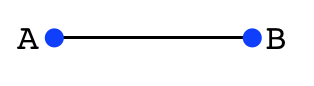
\includegraphics [scale=0.4] {PI_1a.png} \end{center}

The tools we have are a straight-edge and a compass.  The compass is collapsible, meaning that it cannot be used to transfer distances since it loses its setting when lifted from the page.  As we'll see in the next part, this is a problem with a solution.

Euclid was smart enough to know about compasses and how to set them.  The idea he had was this:  to make the fewest possible assumptions.  A non-collapsible compass was a luxury he didn't need, since he could accomplish the same end without it, as we will see.

The first step is to draw two circles on centers $A$ and $B$.
\begin{center} 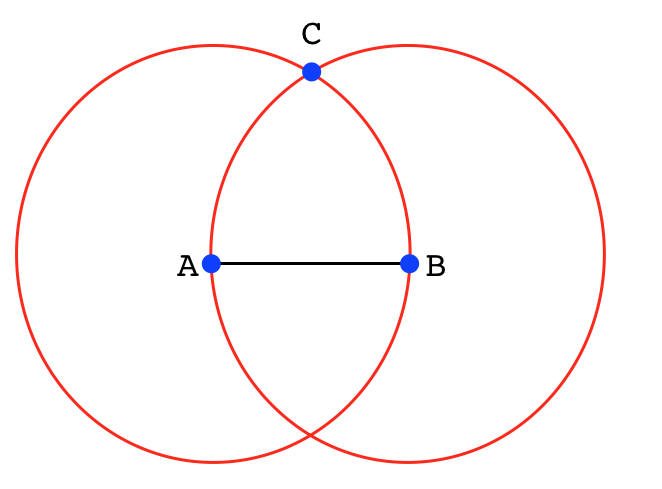
\includegraphics [scale=0.3] {PI_1b.png} \end{center}

The circles are drawn with each radius equal to the line segment $AB$.  It is a property of circles that all points on the circle are at the same distance from the center.  Thus all points on the left-hand circle are equidistant from $A$, and all points on the second one are equidistant from $B$.  

Therefore, the point $C$  where the circles cross is equidistant from \emph{both} $A$ and $B$.

For this, we don't really need the entire circles, just the part where the arcs cross at $C$.

\begin{center} 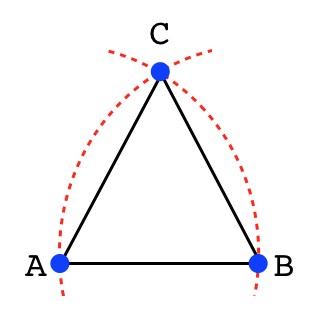
\includegraphics [scale=0.4] {PI_1c.png} \end{center}

Now use the straight edge to draw $\triangle ABC$.  Since $AC = AB$ and $BC = AB$, we know that $AC = BC$.  The triangle is equilateral.

We put a little box to show that the proof is complete.

$\square$

The proof doesn't stand on its own.  We used one definition (D) and a common notion (CN).

$\circ$ \ D I.15  all radii of a circle are equal.

$\circ$ \ CN I.1  things which equal the same thing also equal one another.

If we look again at the figure, and label the other point where the circles cross as $D$:
\begin{center} 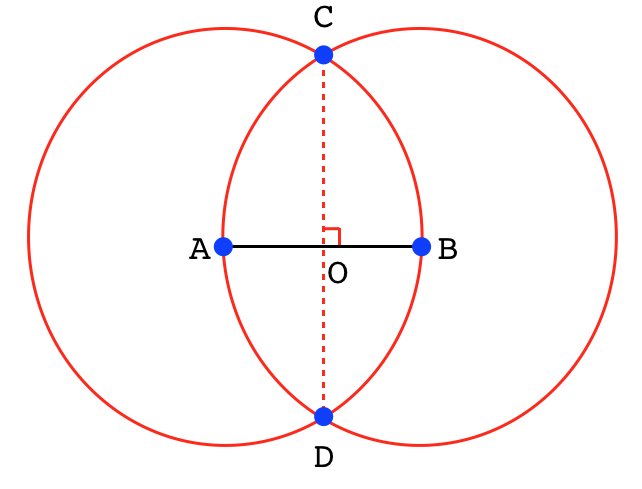
\includegraphics [scale=0.3] {PI_1d.png} \end{center}

Note:  $CD$ is the perpendicular bisector of $AB$.  Euclid doesn't have the tools to prove that yet, so he leaves it for now.

If desired, we could draw on tools from the last chapter.  Clearly $\triangle ABC$ and $\triangle ABD$ are equilateral triangles with sides of the same length.  From that, we deduce that $\triangle ACD$ and $\triangle CBD$ are isosceles.  And from that, we can easily prove that all four small triangles with $O$ as a vertex are equal and therefore right angles.  

We leave this as an exercise.

\subsection*{Prop. I.2}
To place a straight line equal to a given straight line with one end at a given point.

We will construct a line segment at $A$ equal in length to $BC$ (left panel).  The first thing is to draw the line segment $AB$ and construct an equilateral triangle on it (right panel).   
\begin{center} 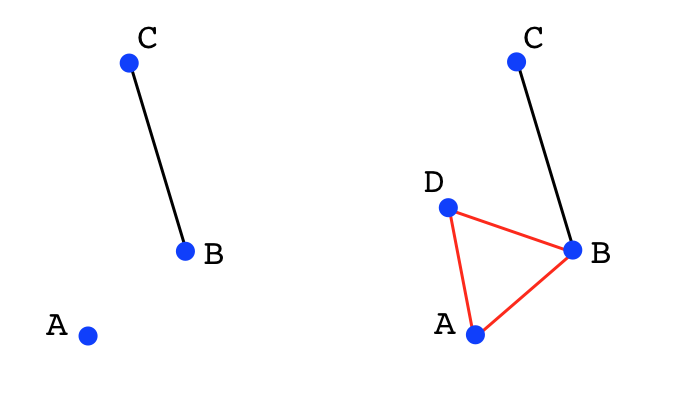
\includegraphics [scale=0.4] {PI_2b.png} \end{center}

We know how to do this (from $P I.1$).  

Next, construct a circle on center $B$ with radius $BC$ and extend the line segment $DB$ to point $G$.  

Then, construct a circle on center $D$ with radius $DG$ and extend $DA$ to that circle at point $L$.  

We have:

\begin{center} 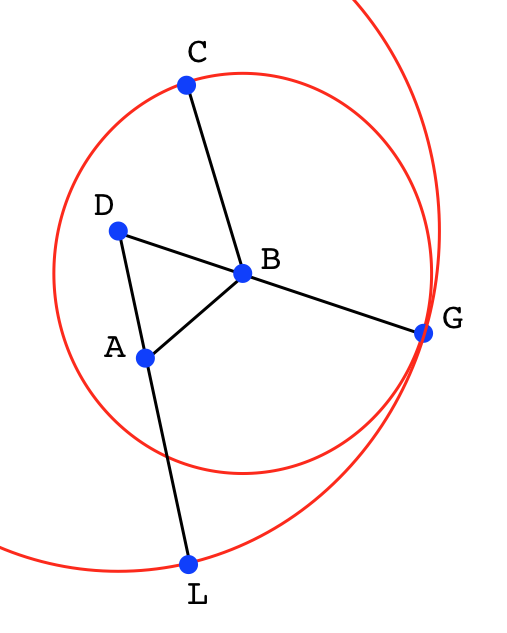
\includegraphics [scale=0.3] {PI_2c.png} \end{center}

As common radii of the circle on center $B$, we have $BC = BG$.  

As common radii of the circle on center $D$, we have $DL = DG$.  

As sides of an equilateral triangle, we have $DA = DB$.

We use CN $I.3$:  if equals are subtracted from equals, then the remainders are equal.  Thus, $AL = BG$.  But we had above that $BC = BG$.  Therefore, $AL = BC$, by CN $I.1$.  

Q.E.D. or "quod erat demonstrandum", in Latin

And in the original Greek \emph{the very thing it was required to have shown.}

$\square$

Note in passing, the orientation is determined by $AB$.  We have not shown how to transfer the length with an arbitrary orientation.  We will solve this next.

\subsection*{Prop. I.3}
To cut off the lesser of two unequal straight lines from the greater.

\begin{center} 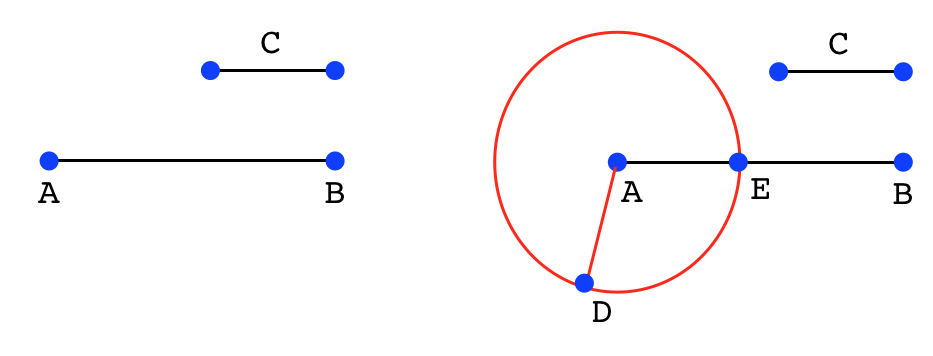
\includegraphics [scale=0.4] {PI_3a.png} \end{center}

In the left panel, we have the line segment $AB$ and a smaller one just labeled $C$.  To do the construction, use the method of P $I.2$ and transfer $C$ to point $A$, forming $AD$.  

Next, use $AD$ as the radius of a circle on center $A$.  Then, $AE = AD$, but $AD = C$.  Hence \[ BE = AB - AE = AB - AD = AB - C \]

as required.

$\square$

At this point, we have a method to mark off a given length from a larger length, even though all we have is a collapsing compass.  Therefore, going forward, we can act as if we have a standard compass, that holds its setting after being lifted from the paper.

We also have the means to an important \emph{trichotomy}.  Comparing two line segments, one of three things must be true:  either the first is smaller than the second, they are equal, or the second is smaller than the first.

\subsection*{Prop. I.4}

If two triangles have two sides equal to two sides respectively, and have the angles contained by the equal straight lines equal, then they also have the base equal to the base, the triangle equals the triangle, and the remaining angles equal the remaining angles respectively, namely those opposite the equal sides.

\begin{center} 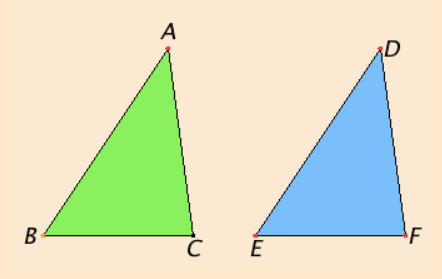
\includegraphics [scale=0.4] {PI_4a.png} \end{center}

This is not a construction, unlike the previous three propositions.  It is a method for proving congruence (equality) of two triangles 
\[ \triangle ABC \cong \triangle DEF \]

Elsewhere in this book we would call the method SAS or \emph{side angle side}.  Given that $AB = DE$ and $AC = DF$ and that the angles between them at the vertices $A$ and $D$ are also equal, the two triangles are congruent:  all three angles and all three sides are equal.

This (P $I.4$) is a proof that SAS is correct.

The proof is by superposition.  The facts establish the positions of the points $B$ and $C$, which determines $AB$ and so the angles at vertices $B$ and $C$.

Euclid says that if we lift up $\triangle ABC$ and lay it on top of $\triangle DEF$ then $B$ coincides with $E$ and $C$ coincides with $F$ so $BC = EF$.

$\square$

This seems perhaps a little shaky logically, and it's not a method of proof that Euclid uses much.

But one might instead have taken this proposition as a postulate.  The source, above, says that David Hilbert claims that under the hypotheses of the proposition it is true that the two base angles are equal, and then proves that the bases are equal.

We have used SAS to prove SSS, that all three sides are equal.

\subsection*{Prop. I.5}

In isosceles triangles the angles at the base equal one another, and, if the equal straight lines are produced further, then the angles under the base equal one another.

We proved this theorem in the previous chapter on isosceles triangles.

Euclid's proof of the converse is short and introduces the method of contradiction, or \emph{reductio ad absurdum}.  That is the next proposition.
  
\subsection*{Prop. I.6}

If in a triangle two angles equal one another, then the sides opposite the equal angles also equal one another.

Suppose we have $\triangle ABC$ with equal angles $\beta = \gamma$ at the base (left panel).

\begin{center} 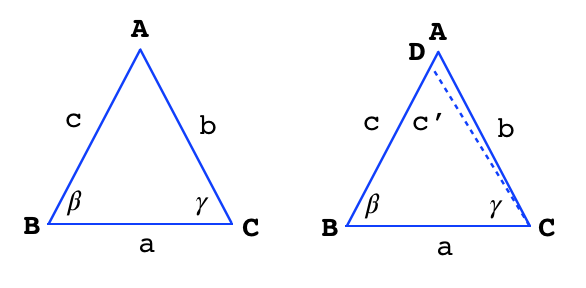
\includegraphics [scale=0.5] {PI_6b.png} \end{center}

We will assume that the two sides $b$ and $c$ are not equal.  Then one of them is greater.  Let $c$ be greater, then cut off $b$ from $c$ at point $D$ such that the new length $c' = b$.

The new triangle has sides $c'$ and $a$, which flank angle $\beta$, while for the original we have side $b$ and side $a$ flanking $\gamma$.   But we constructed $c' = b$, are given that $\beta = \gamma$, and the side $a$ is common.  

Therefore the $\triangle DBC \cong \triangle ACB$ by SAS.

But this means that the less equals the greater, which is absurd. 

Therefore $c$ cannot be unequal to $b$.  It therefore equals it.

Our original assumption that $b$ does not equal $c$ must be false.

$\square$

\subsection*{Prop. I.9}

To bisect a given angle.

\begin{center} 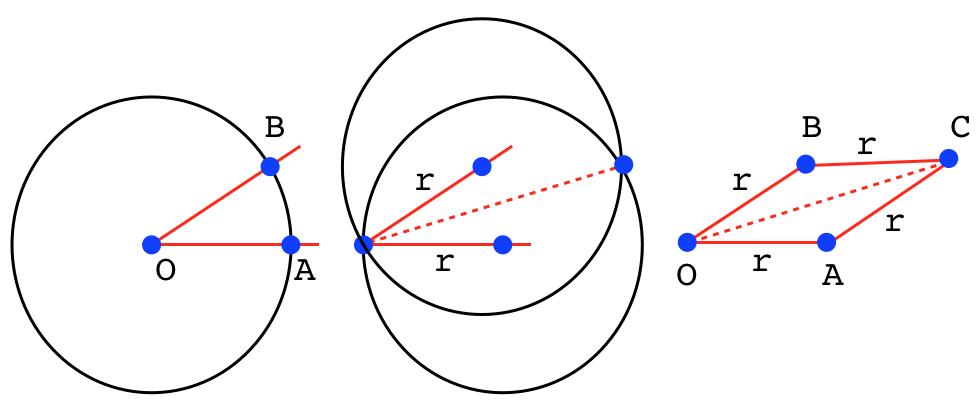
\includegraphics [scale=0.4] {PI_9a.png} \end{center}

As radii of a circle on center $O$, we first find points $A$ and $B$ equidistant from $O$ (left panel).  Let that distance be $r$.

As radii of circles on the centers $A$ and $B$ that pass through $O$ (so the radius is equal to $r$), we find $C$ equidistant from $A$ and $B$ (middle panel), with radius also equal to $r$.

Thus, $OA = OB = AC = BC$ (right panel).  

So $\triangle OAC \cong \triangle OBC$.

Therefore $\angle BOC$ is equal to $\angle AOC$ and the given angle is bisected.

$\square$


We will do three more.  They are short, sweet and powerful.  

In these examples, we use letters late in the alphabet ($s, t, u, v$) for angles, while $a, b, c$ are labels for sides.

\subsection*{Prop. I.16}

In any triangle, if one of the sides is produced (extended), then the exterior angle is greater than either of the interior and opposite angles.

\begin{center} 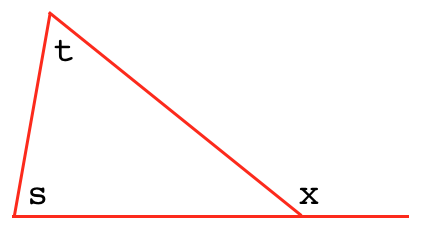
\includegraphics [scale=0.4] {PI_16a.png} \end{center}

The claim is that the exterior angle $x$ is greater than either of the interior angles:  $s$ or $t$.  

Find the midpoint of the side opposite $s$ and draw the indicated line segment (right panel, below), so that the two segments marked with black arrows are equal, as well as the segments marked with blue arrows.  
\begin{center} 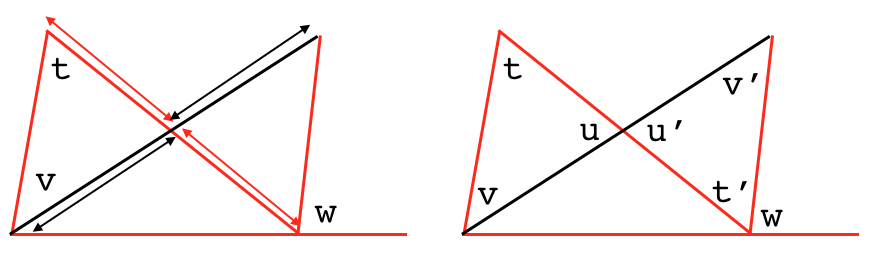
\includegraphics [scale=0.4] {PI_16b.png} \end{center}

By SAS and the vertical angle theorem, the two smaller triangles to the left and right with dotted lines are congruent, as indicated in the right panel by the labels on the angles:  $t = t', u = u', v = v'$.

The original external angle $x$ is seen to be composed of $t' + w$, that is
\[ x = t' + w \]
so clearly (the whole is greater than its parts):
\[ x > t' \]
but since $t = t'$:
\[ x > t \]

We can make a similar construction and proof for angle $s$.

The exterior angle is greater than either of the interior and opposite angles.

$\square$

\subsection*{external angle theorem}
The external angle theorem is extremely useful, so let's take a break from Euclid and prove it now.  The proof is simple for us:
\begin{center} 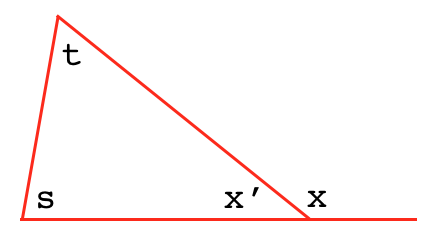
\includegraphics [scale=0.4] {PI_16c.png} \end{center}

As supplementary angles, $x + x' = 180$ degrees.  As the three angles of a triangle, $s + t + x' = 180$ degrees as well.  Things equal to the same thing are equal to each other:
\[ x + x' = s + t + x' \]
\[ x = s + t \]

The question of why Euclid doesn't use supplementary angles here is complicated.  For now it is enough to say that he just doesn't.

\subsection*{Prop. I.18}

In any triangle, a greater side is opposite a greater angle.

\begin{center} 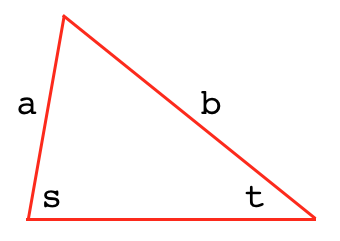
\includegraphics [scale=0.4] {PI_18a.png} \end{center}

Given $b > a$, mark off $a$ on $b$.

\begin{center} 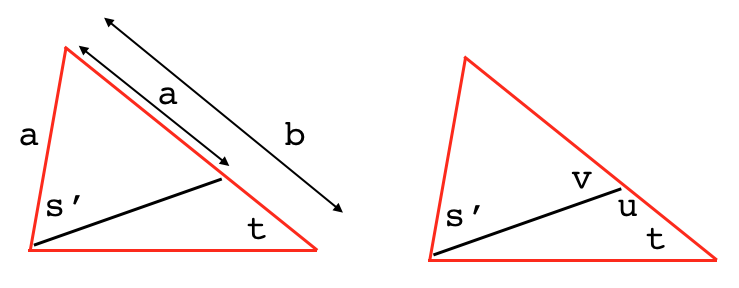
\includegraphics [scale=0.4] {PI_18b.png} \end{center}

By the external angle theorem (I.16)
\[ v > t \]

But $v = s'$ (by isosceles $\triangle$, $I.5$) so 
\[ s' > t \]
And since $s > s' $
\begin{center} 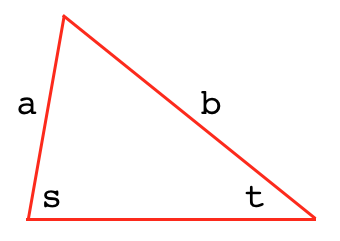
\includegraphics [scale=0.4] {PI_18a.png} \end{center}
\[ s > t \]

$\square$

We get the converse almost for free.

\subsection*{Prop. I.19}

In any triangle, a greater angle is opposite a greater side.

\begin{center} 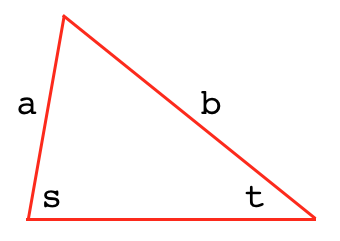
\includegraphics [scale=0.4] {PI_18a.png} \end{center}

We are given $s > t$ and want to prove $a < b$.  We proceed by considering the other possibilities.

It cannot be that $a = b$ because then $s = t$ by isosceles $\triangle$ ($I.5$), but we are given $s > t$.

So then suppose $a > b$.  By the previous proposition ($I.18$), we would have that $t > s$.  But this is again contrary to what we were given.  Hence $b > a$.

$\square$

We have made use of the trichotomy from before, that there are only three possibilities:
\[ a < b, \ \ \ \ \ \ a > b, \ \ \ \ \ \ a = b \]

This applies to line segments and angles as well as many other things.

This is enough of the \emph{Elements} to give us a good taste of the basics of Greek geometry of lines and triangles, and methods of proof.  There is more to come:  Pythagoras, and circles with their arcs and tangents.

\end{document}